\documentclass{standalone}
\usepackage{tikz}
\usetikzlibrary{shapes.callouts}
\usepackage{tkz-fct}
\usepackage{tkz-euclide}
\usepackage{color}
\renewcommand*\familydefault{\sfdefault}
\usepackage{sansmath}
\usepackage{amsmath}

\sansmath
\definecolor{gray75}{gray}{0.75}
\begin{document}
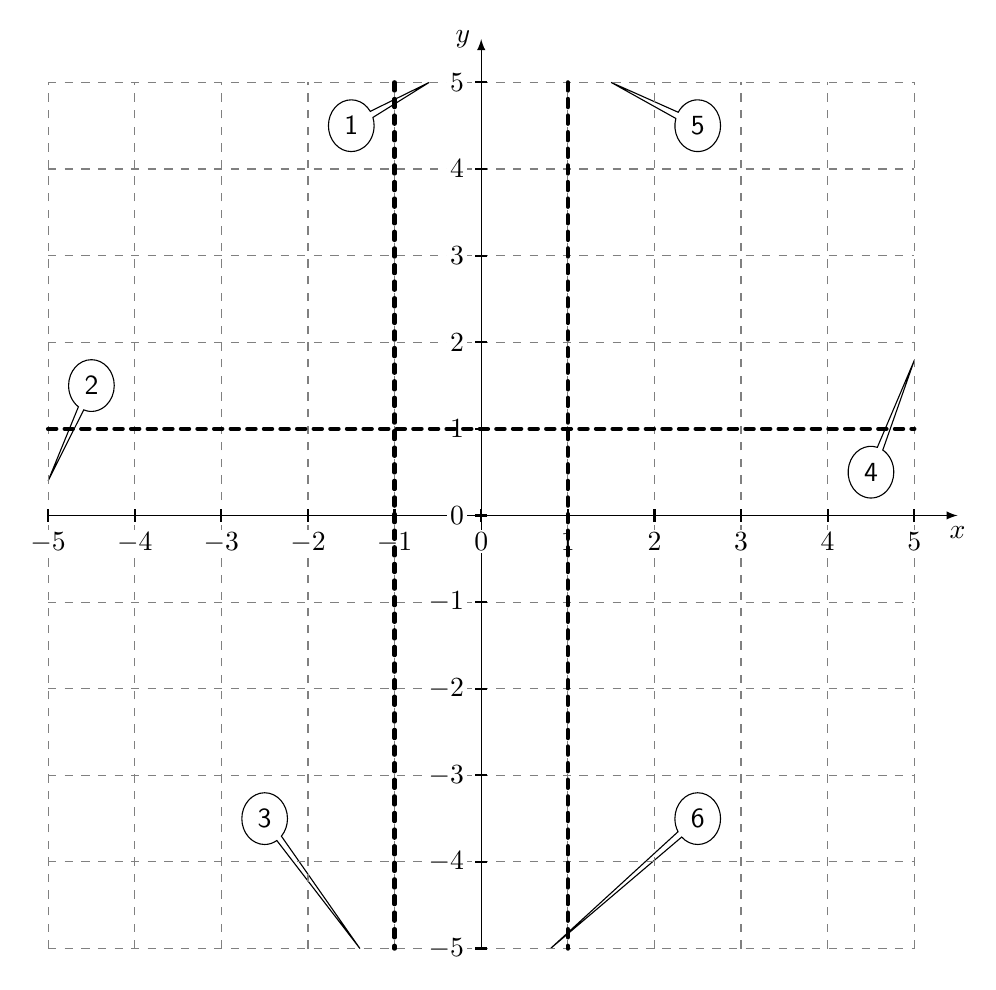
\begin{tikzpicture}[scale=1.1]
  \node[ellipse callout,draw,callout absolute pointer={(-0.6,5)}] at
  (-1.5,4.5) {1}; %
  \node[ellipse callout,draw,callout absolute pointer={(-5,.4)}] at
   (-4.5,1.5) {2}; %
  \node[ellipse callout,draw,callout absolute pointer={(-1.4,-5)}] at
    (-2.5,-3.5) {3}; %
  \node[ellipse callout,draw,callout absolute pointer={(5,1.79)}] at
     (4.5,0.5) {4}; %
  \node[ellipse callout,draw,callout absolute pointer={(1.5,5)}] at
     (2.5,4.5) {5};
  \node[ellipse callout,draw,callout absolute pointer={(0.8,-5)}] at
     (2.5,-3.5) {6};
  \tkzInit[xmin=-5, xmax=5,ymin=-5,ymax=5]
  \begin{scope}[dashed]
    \tkzGrid
  \end{scope}
  \tkzDrawX[label={$x$}]
  \tkzDrawY[label={$y$}]
  \tkzLabelX
  \tkzLabelY
  \tkzFct[line width = 2pt,domain=-5:-1.1]{(2/1.75*(x-0.5)*(x+3.5)/(x**2-1))}
   \tkzFct[line width = 2pt,domain=-0.9:0.9]{(2/1.75*(x-0.5)*(x+3.5)/(x**2-1))}
  \tkzFct[line width = 2pt,domain=1.1:5]{(2/1.75*(x-0.5)*(x+3.5)/(x**2-1))}
 \tkzDefPoint(-5.0,1){A}
  \tkzDefPoint(5.0,1){B}
  \tkzDrawSegment[style=dashed,line width = 1.5pt](A,B)
  \tkzDefPoint(-1,5){A}
  \tkzDefPoint(-1,-5){B}
  \tkzDrawSegment[style=dashed,line width = 1.5pt](A,B);
\tkzDefPoint(1,5){A}
  \tkzDefPoint(1,-5){B}
  \tkzDrawSegment[style=dashed,line width = 1.5pt](A,B);

\end{tikzpicture}
\end{document}